\documentclass{article}
\usepackage{tikz, comment}
\usepackage{pifont}
\usepackage{fontspec}
\usetikzlibrary{arrows, decorations.markings, decorations.pathreplacing}
\begin{comment}
:Title: Not defined yet
:Slug: No name yet

Description Here.........
\end{comment}
\begin{document}\centering 

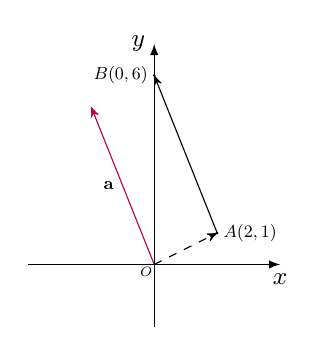
\begin{tikzpicture}[>=latex,xscale=.5*0.8, yscale=.5*0.8][font=\sf\small] 

%\draw[xstep=1cm,ystep=1cm,color=gray!80] (0, -1) grid (8, 8);

    	\foreach \x in {}
     		\draw (\x,2pt/8) -- (\x,-2pt/8)
			node[anchor=north] {\tiny$\x$}
			;

    	\foreach \x in {}
     		\draw (\x,2pt/1) -- (\x,-2pt/1)
			node[anchor=south] {\tiny$\x$}
			;
    	\foreach \y in {}
     		\draw (-2pt/1,\y) -- (2pt/1,\y)
			node[anchor=east] {\tiny $\y$}
			;

\draw[->] (-4, 0) -- (4, 0)node[below] {$x$} ;
\draw[->] (0, -2) -- (0, 7)node[left] {$y$} ;

\draw[fill] (2,1) circle(0.02)node[right, scale=0.7] {$A(2,1)$};
\draw[fill] (0,6) circle(0.02)node[left, scale=0.7] {$B(0,6)$};

\draw[dashed, ->, >=stealth'] (0, 0) -- (2,1); %A
%\draw[dashed, ->, >=stealth'] (0, 0) -- (0,6); %B

\draw[->, >=stealth'] (2,1)--(0,6);


\draw[purple, ->, >=stealth'] (0, 0) -- (-2, 5)node[black, left, midway, pos=0.5, xshift=-1, yshift=0, scale=0.7]{$\bf a$};

\node[scale=0.7] at (-0.2/0.8, -0.2/0.8) {\scriptsize$O$};

\end{tikzpicture}
\end{document}